
\subsection{Splitting a node}

\begin{figure}
    \centering
    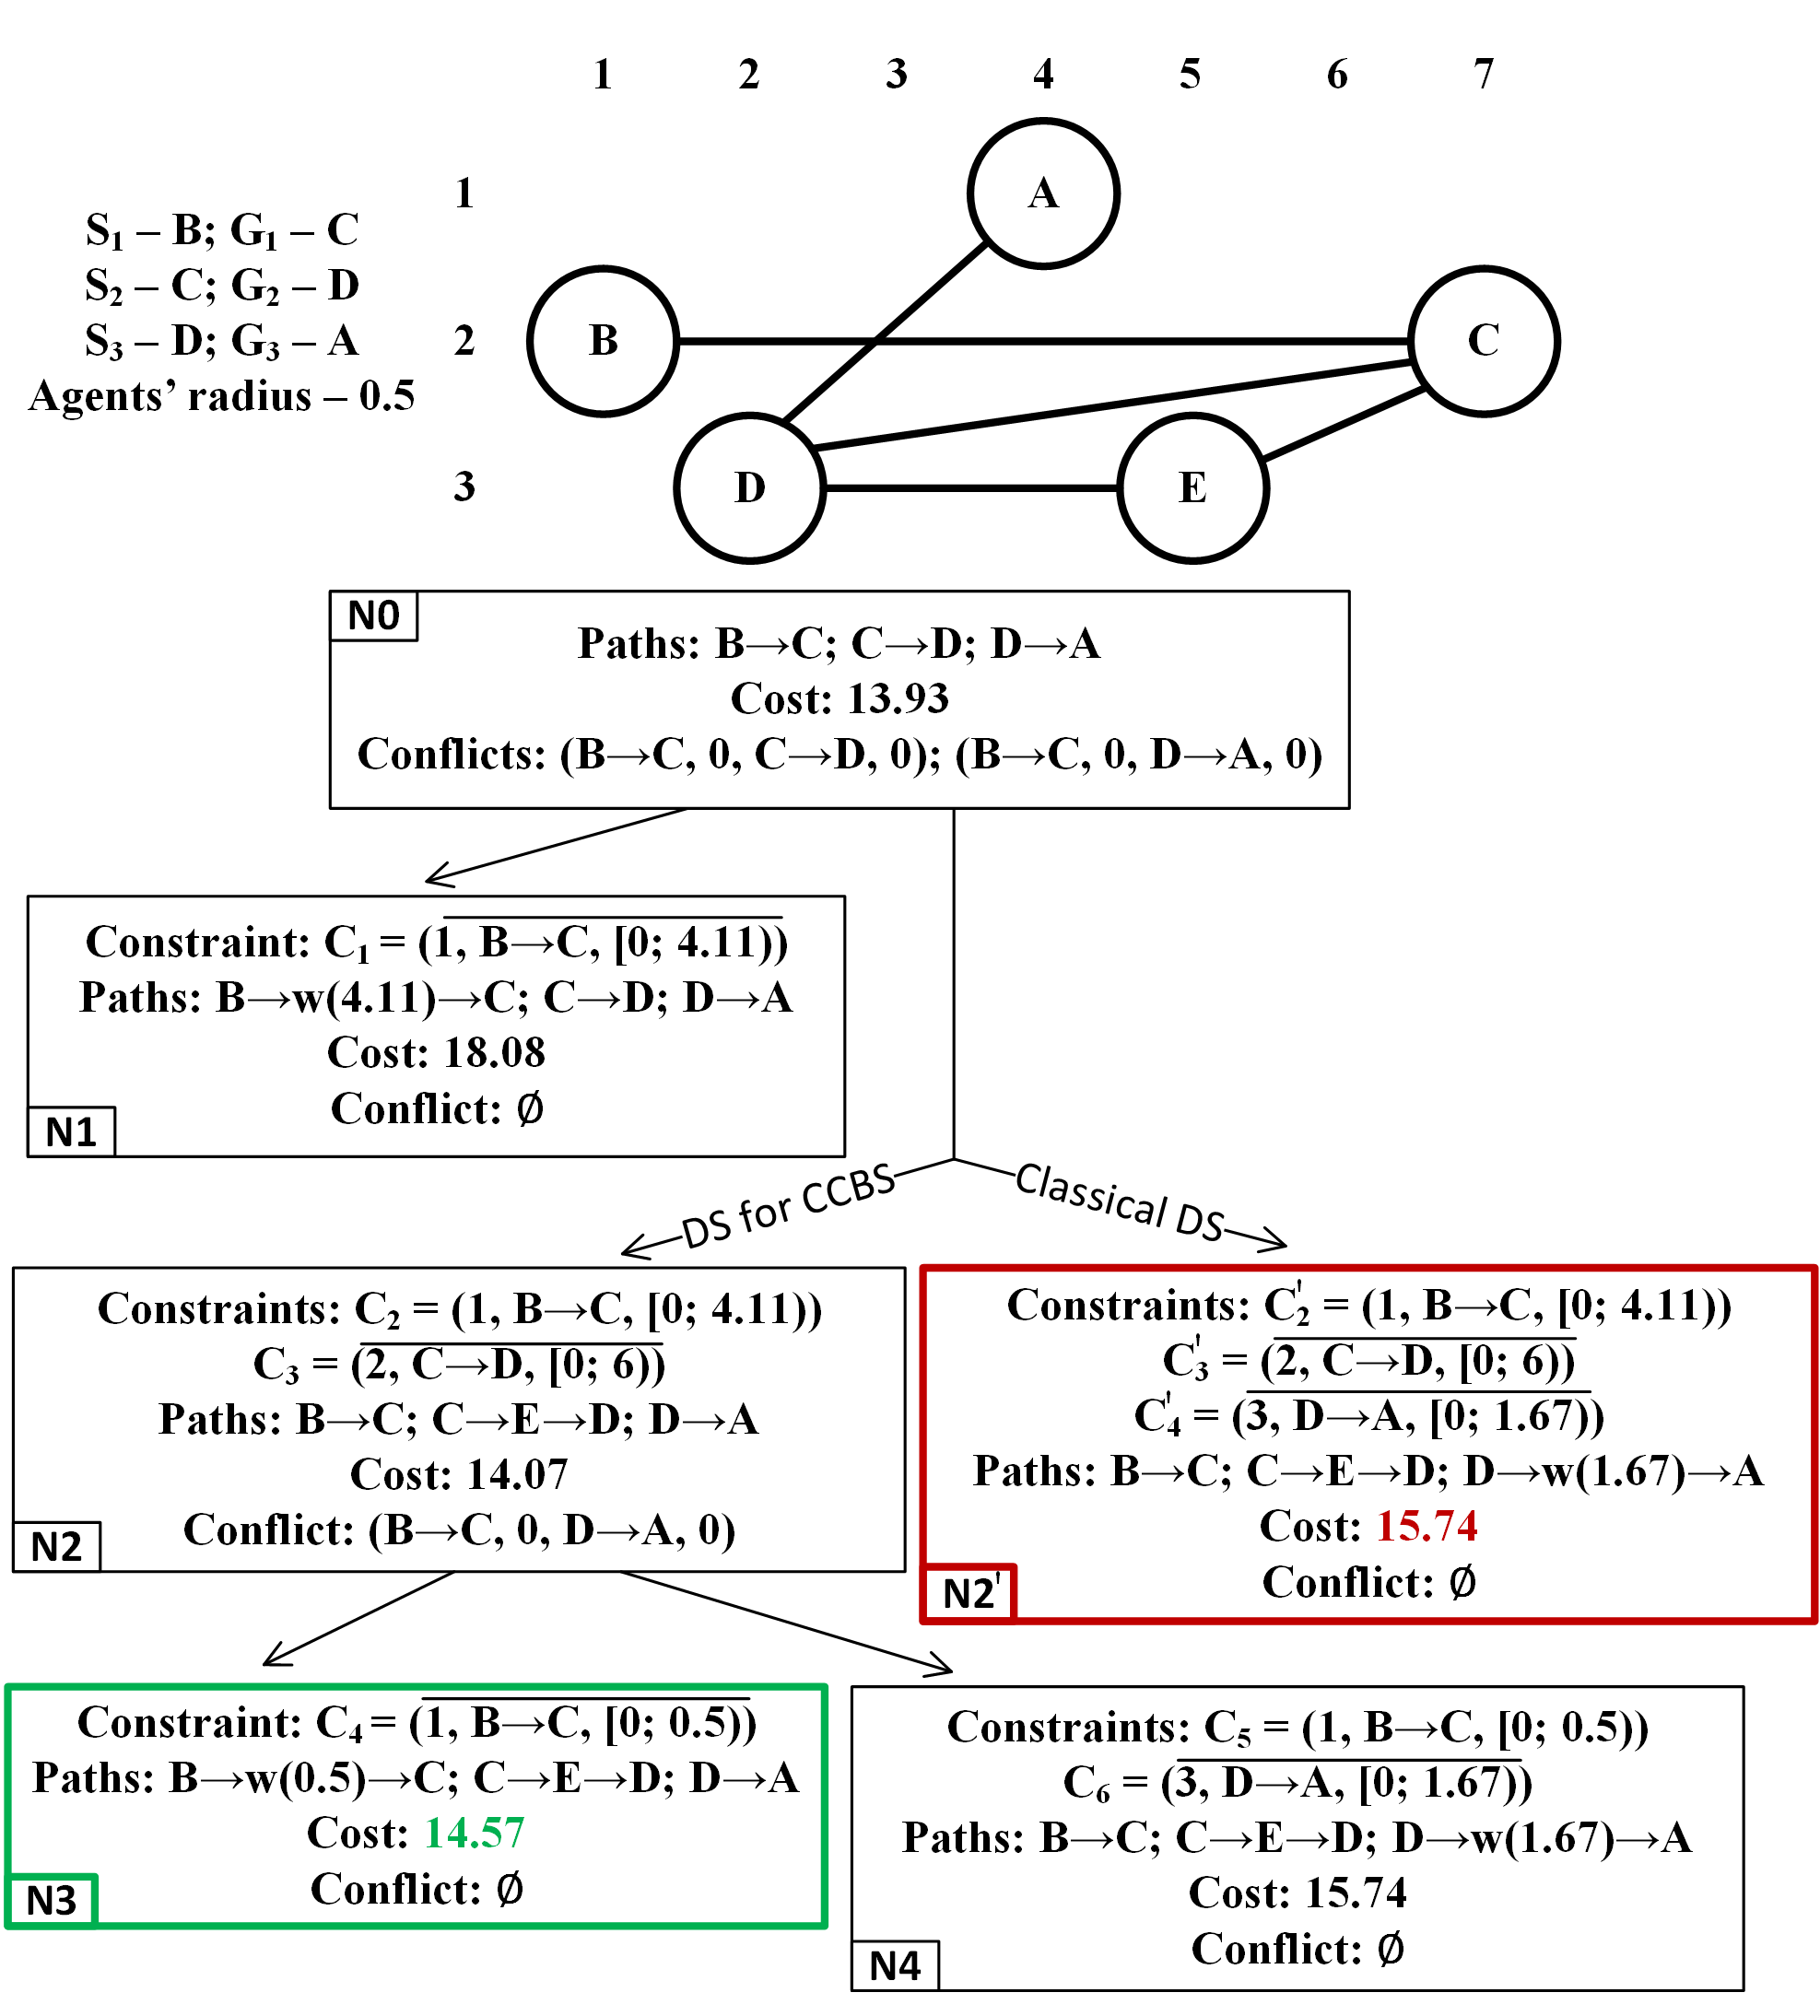
\includegraphics[width=\columnwidth]{Example1.png}
    \caption{The difference between disjoint splitting for classical \mapf and \mapfr.}
    \label{fig:ds_for_ccbs}
\end{figure}

\konstantin{I altered the text in this section following the discussion on what kind of negative constraints can one add to a positively constrained \ct node. Please check/edit.}

When splitting a \ct node $N$ in \cbsds and imposing a positive constraint, $C=(i, x, k)$ on one of its children, $N'$ one may simultaneously add to $N'$ the corresponding negative constraints $C_j=\overline{(j, x, k)}$ that involve other agents $j: j \neq i$. The question now is -- in case $C$ is a \ccbs positive constraint, i.e. $C=(i, a_i, [t_i, t_i^u))$ what kind of negative constraints on the other agents can we add to $N'$? Obviously, one can add a negative constraint on the action $a_j$ of the agent $j$ that led to the split (that is what regular \ccbs would do): $C_{neg_1}=(j, a_j, [t_j, t_j^u))$. \konstantin{Actually, I have no proper explanation why we need to add this constraint except: this is what CCBS does.} Can we add to $N'$ other negative constraints that correspond to the timed actions that have conflicts with $a_i$ at $N$? 

To answer this question consider an example depicted on Fig.~\ref{fig:ds_for_ccbs}. A conflict between the 1st and the 2nd agent is chosen to perform a split at the root \ct node. Its descendant $N1$ is created with the negative constraint $C_1$ prohibiting the action $B \rightarrow C$ to be performed within the interval $[0, 4.11)$. The corresponding positive constraint $C_2$ is added to its other descendant $N2'$. Assume now that we immediately add to $N2'$ the negative constraint $C_4'$ that prohibits the 3rd agent to perform a move $D \rightarrow A$ as this move is also in conflict with the move we are splitting on, i.e. $(B \rightarrow C, 0)$. Indeed, the individual planner will find a set of individual plans for the agents that respect the constraints of $N2'$, including $C_4'$. Moreover, the resulting set of plans is conflict-free and will be returned as the solution of \mapfr. However this solution is not optimal. To find an optimal one one must not add $C_4'$ immediately to the descendant of $N_0$ that contains the positive constraint $C_2$, but rather discover this conflict later on as shown on the left part of the \ct tree.

The above-said clearly illustrates that adding extra negative constraints to a positively constrained \ct node is not straightforward.

In logic terms, a positive \ccbs constraint says there must exists a time $t$ in the interval where agent $i$ will do $a_i$, so the negative constraints on the other agents will be that they must not create a plan that blocks $i$ from performing $a_i$ in \emph{its entire time range}. More formally:

\textit{Assume that a conflict $(a_i, t_i, a_j, t_j)$ between the agents $i$ and $j$ is found, corresponding unsafe intervals - $[t_i, t_i^u), [t_j, t_j^u)$ - are computed and a \ct node $N$ is disjointly splitted, i.e. its two descendants are created: $N'$ with a negative constraint $C_{neg}=\overline{(i, a_i, [t_i, t_i^u))}$ and $N''$ with a positive constraint $C_{pos}=(i, a_i, [t_i, t_i^u))$. Then only those additional negative constraints $C_{neg'}=\overline{(m, a_m, [t_m, t_i^m))}$ involving agents $m: m \neq i, j$ can be added to $N''$ that satisfy:.
\[
\forall t\in [t_m, t_m^u), t'\in [t_i, t_i^u): (a_m, t, a_i, t') ~~~ \text{is a \ccbs conflict}
\]
}

Indeed, identifying such actions, $a_m$, and computing the intervals $[t_m, t_m^u)$ is not trivial and requires additional processing. Moreover the standard \ccbs machinery, i.e. computing the unsafe interval of an action $a_m$ against a timed-action $(a_i, t_i)$ is not enough as now one have to compute an unsafe interval against another interval, which is part of a positive constraint -- $[t_i, t_i^u)$. In our experiments we did not perform such computations and did not add extra negative constraints to a positively constrained node (except the negative constraint on the action that caused the split, as described above).

%\roni{I don't think this is true. One can add a negative constraint saying that the other agent must not perform actions that will prevent $i$ from performing $a_i$ in all the time interval in which it must perform $a_i$. 
%In logic terms, the positive constraints say there must exists a time $t$ in the interval where agent $i$ will do $a_i$, and the negative constraints on the other agents will be that they must not create a plan that blocks $i$ from performing $a_i$ in its entire time range. So, this would be something like allowing an action of another agent to be performed only if its unsafe interval with $a_i$ does not fully contain the time interval in which $a_i$ must perform its action.}\konstantin{I did not quite get it. Did you go through an example that supports that claim (it is in the next paragraphs)? Do you agree with that example?}
%\roni{Consider a timed action $(a_m,t_m)$ such that the unsafe interval 
%with $a_i$ is $[t_i,t_i^u)$. 
%Any solution under the CT node $C''$ cannot have the timed action $(a_m,t_m)$, since otherwise the positive constraint cannot be satisfied.}\konstantin{Now I got it. Need to think of it.}








%This is natural in discrete-time domains, as occupying $x$ at time step $k$ by a particular agent necessarily implies that no other agent may be at $x$ at the same time step. When constraints are associated with continuous time intervals this is not longer the case.



%One can also imagine cases when adding extra negative constraints to a positively constrained \ct node leads to not finding a solution at all although it exists and will be found if the disjoint splitting is done in appropriately. 
%\roni{I don't understand the paragraph above}\konstantin{It's here to say smth. like this. In the Example we showed how addining additional negative constraints may lead to finding non-optimal solution. One can also construct another example, showing that immediately adding ``additional'' negative constraints may also lead to not finding a solution at all for this node. I agree that it needs a proper re-phrasing or (possible) ruling this out.}



